\section{Part D: Distribution Comparison with KS-Test}
\begin{itemize}
    \item Compare the empirical distributions of sample means (from power law vs. uniform) using the Kolmogorov--Smirnov (KS) test.
    \item Discuss whether the KS-test supports the theoretical expectation that both sample mean distributions should approximate normality under the CLT. And investigate how the power of the KS-test changes as the number of sample means increases ($10$, $100$, $1000$).
\end{itemize}
-----\\

I performed one-sample KS tests comparing each distribution of sample means to its theoretical normal distribution. The implementation is shown below:

\begin{verbatim}
def ks_test_theoretical_normal(sample_means: np.ndarray, theoretical_mu: float,
                                          theoretical_se: float) -> tuple:
    """
    Performs KS test comparing sample means to their theoretical normal distribution.
    
    :param sample_means: Array of sample means
    :type sample_means: np.ndarray
    :param theoretical_mu: Theoretical mean from CLT
    :type theoretical_mu: float
    :param theoretical_se: Theoretical standard error from CLT
    :type theoretical_se: float
    :returns: Tuple of KS statistic, p-value
    :rtype: tuple
    """
    ks_stat, p_value = stats.kstest(sample_means, 
                                    lambda x: stats.norm.cdf(x, 
                                                             loc=theoretical_mu, 
                                                             scale=theoretical_se))
    
    return ks_stat, p_value
\end{verbatim}
\begin{center}
\textbf{Figure 20:} KS test function comparing sample means to theoretical normal distribution.\\
\end{center}

The one-sample KS test results for each distribution at different replicate sizes are tabulated below. Each test compares the empirical distribution of sample means to the theoretical normal distribution (Uniform: $N(0.75, 0.029^2)$, Pareto: $N(0.769, 0.140^2)$):
\begin{center}
    \textbf{KS Test Results: Sample Means vs Theoretical Normal Distribution}
    \vspace{0.5em}
    \begin{tabular}{lcc|cc}
    \toprule
    & \multicolumn{2}{c|}{Uniform Distribution} & \multicolumn{2}{c}{Power Law Distribution} \\
    \textbf{Replicate Size} & \textbf{KS Statistic} & \textbf{p-value} & \textbf{KS Statistic} & \textbf{p-value} \\
    \midrule
    10 & 0.240 & 0.537 & 0.160 & 0.925 \\
    100 & 0.114 & 0.135 & 0.221 & 8.92e-5 \\
    1000 & 0.016 & 0.945 & 0.059 & 0.002 \\
    \bottomrule
    \end{tabular}
\end{center}

The Uniform distribution shows support for normality across each replicate size, with all the p-values being above 0.05, failing to reject the null hypothesis; the sample means ought to be following a Normal distribution. The KS statistics decreases from 0.240 to 0.016 with increasing replicates, so the agreement with the theoretical Normal distribution is increasing with greater numbers of sample means, as CLT would suggest.\\

The Pareto distribution reveals the effect of heavy tails on the KS test's power. At replicate size 10, the test fails to reject ($p=0.925$) with a KS statistic of 0.160. This signals the limits of the KS test's power at smaller sample sizes because the KS stat at replicate size 10 is 0.16, which is larger than at replicate size 1000, despite the p-value at replicate size 1000 being significant while the other is not. For this reason, the KS test alone is not as powerful until sample size and statistical power at that sample size are taken into account, because in the case of size 10, the null could be false, but the test does not have enough power at this scale to detect it, whereas at size 1000 the test has so much power that it can detect any of the remaining deviations.\\

We see at size 100, the KS statistic actually increases to 0.221 and becomes highly significant ($p=8.92 \times 10^{-5}$), rejecting the null hypothesis. This increase shows that with 100 replicates, the KS test has enough power at this scale to detect the sample's disagreement with the Gaussian from the heavy tail's influence on the sample mean distribution. This marks a turning point of the KS test becoming powerful with respect to our observations, and then the increase to size 1000 confirms the convergence, albeit the deviations from Normal behavior are still apparent and detectable by the test.\\

I also went ahead and plotted the convergence of the KS statistics for each distribution across the replicate sizes. Although the plot looks quite simple as a visual, it illustrates pretty well the behavior I just mentioned:

\begin{center}
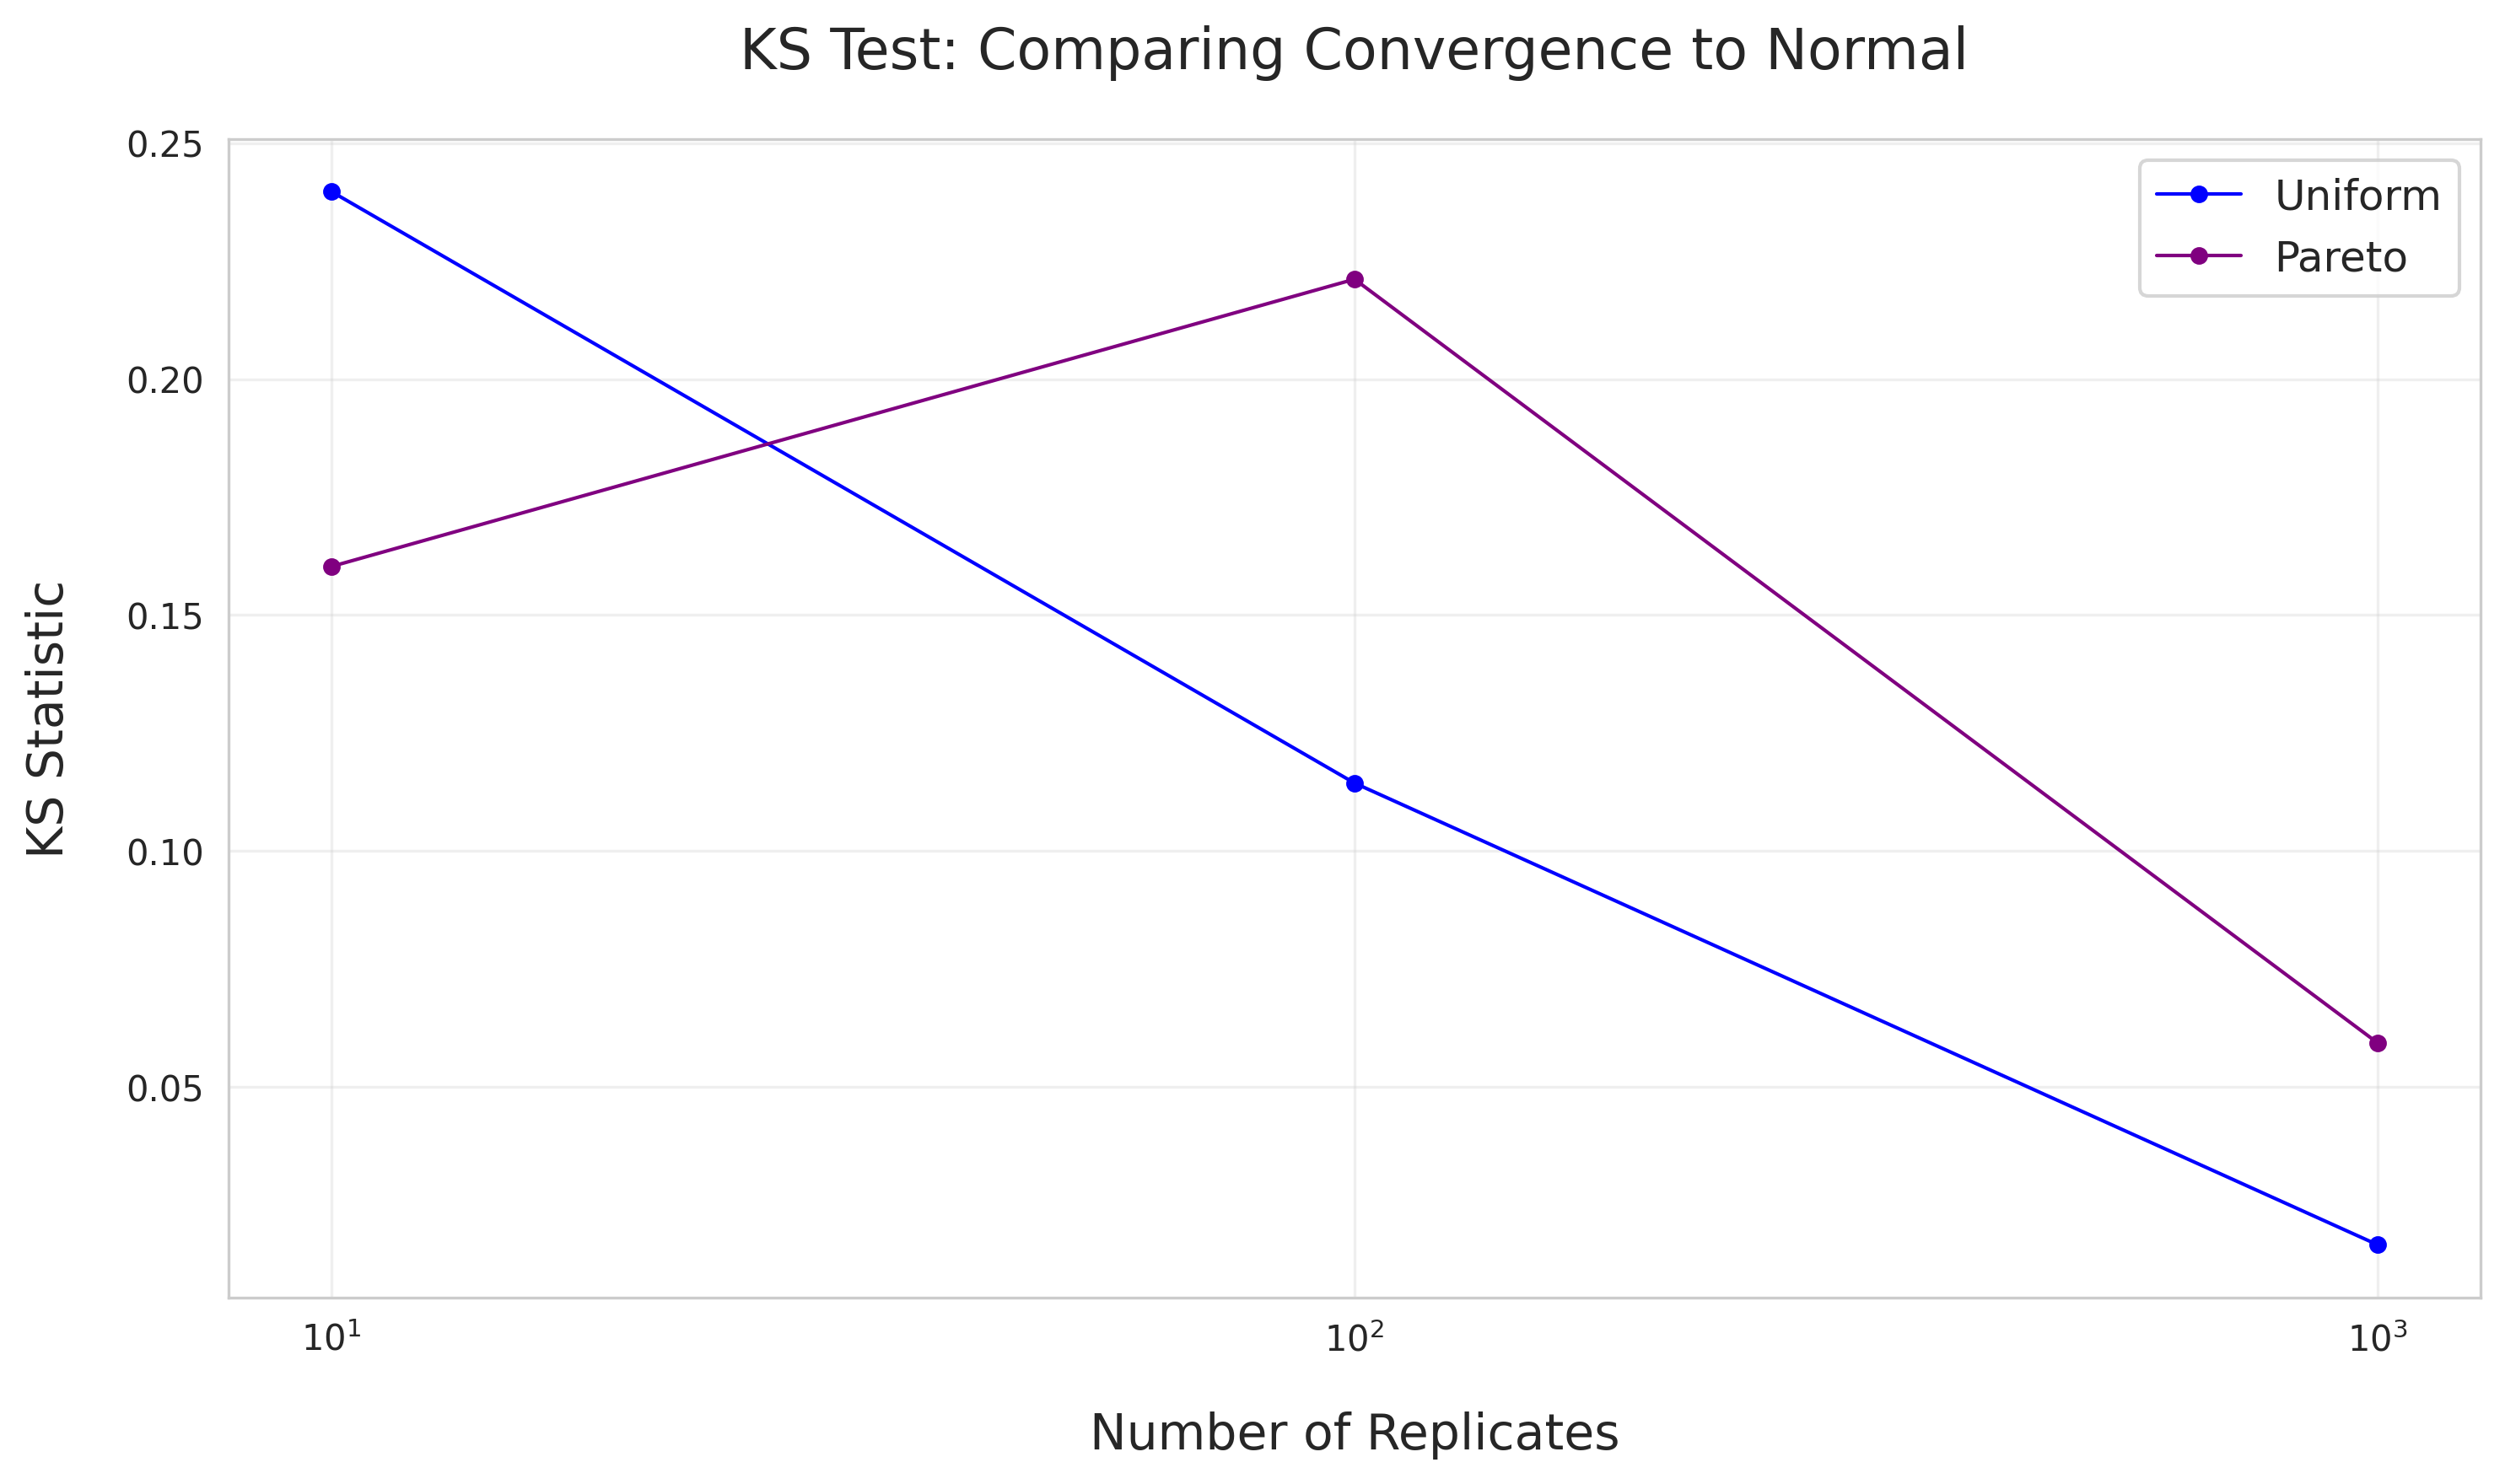
\includegraphics[width=0.95\textwidth]{figures/ks_test_comparison.png}
\textbf{Figure 21:} KS statistics vs replicate size, comparing Uniform and Pareto convergence.
\end{center}

Regarding the Uniform, it shows a consistently decreasing KS statistic, reaching almost zero by size 1000. It has excellent agreement with the Normal simply due to its construction: it doesn't have the issues in collecting sample means with similar behavior like the Pareto does. The Pareto shows an increase from 0.16 to 0.221 between size 10 to 100, and then decreases to 0.059 at size 1000. This is showing that initially, more data to reference the cumulative structure off of shows that deviations were present but undetectable. Then the CLT effect dominates over the tail behaviors of the Pareto causing the occasional extreme sample means.\\

The KS test results support the Central Limit Theorem's prediction that both distributions converge toward the theoretical Normal, though with the caveat that the rate of convergence will be influenced by the particular tail behaviors of the distributions in question.

\newpage